Consider the second-order problem

$$
u''(x) = x u(x),\; x \ge 0
$$

which has a unique solution $u(x)$ when $u$ disappears at infinity. Find this solution numerically, either by solving
it as a boundary value problem or as an initial value problem.

\begin{solution}\ \\\\
    \newpage
    \hfill\vfill
    \pagebreak

    We plot our computed solution $U(x)$ from \texttt{problem\_4a.m} against the built-in \texttt{airy} function
    (denoted $Ai(x)$) below:

    \begin{figure}[h]
        \centering
        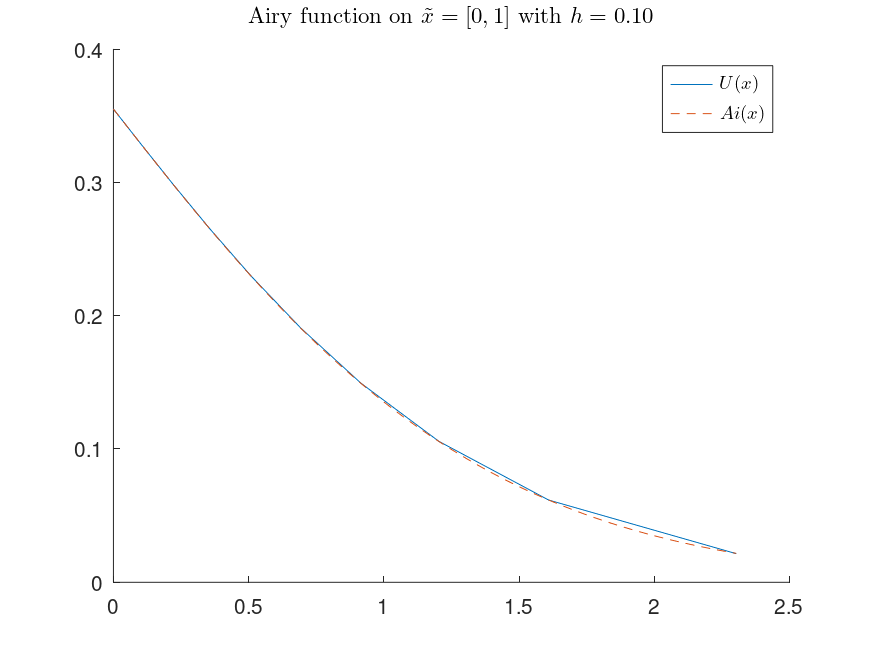
\includegraphics[width=0.85\textwidth]{problem_4a_airy_function.png}
        \caption{Airy equation solution}
    \end{figure}
    \ \\
\end{solution}